\documentclass{article}
\usepackage{caption}
\captionsetup{labelformat=empty}
\usepackage[utf8]{inputenc}
\usepackage{amsmath}
\usepackage{adjustbox}
\usepackage{tabu}
\usepackage{graphicx}
\usepackage{float}
\begin{document}
\section{Kullback-Leibler Divergence}
\subsection{Phonemes and Language Similarity}
\begin{itemize}
	\item[a)]
	A unified phoneme set is constructed from all the different language phonemes. The probability distribution of phonemes is calculated for each corpus with Lidstone smoothing where, $\alpha $= 1. Then 3 test cases are run for different unseen phonemes in different corpus. The probability of unseen phoneme '\$' is calculated in English and French corpus. The probability of another unseen phoneme '1' is calculated in Italian corpus. The test was successful, as in all cases it returns some very little probability value which is not zero. \:
	
	\item[b)]
	    From the bar chart below we can see that the distribution of phonemes in these 4 languages is not uniform at all. In each corpus frequency of some phonemes is much more than the others while there are also such phonemes which frequency is quite low than the remaining.  
		\begin{figure}[H]
            \centering
                \begin{minipage}{.55\textwidth}
                    \centering
                    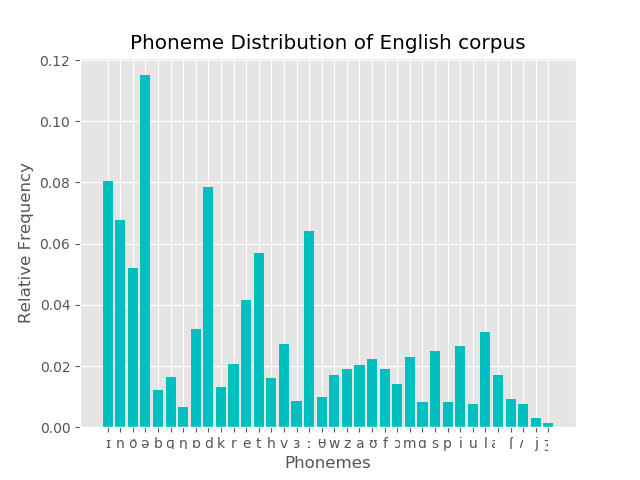
\includegraphics[keepaspectratio=true,scale=0.35]{./source/EX1.1_files/English.png} 
                    \label{fig:prob1_6_2}
                \end{minipage}%
                \begin{minipage}{.5\textwidth}
                    \centering
                    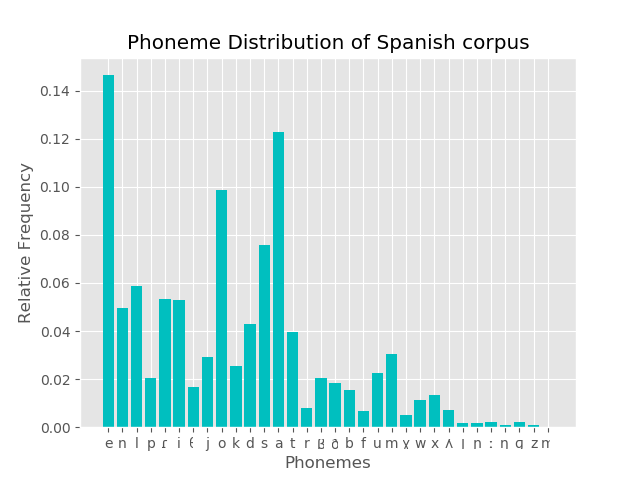
\includegraphics[keepaspectratio=true,scale=0.35]{./source/EX1.1_files/Spanish.png}   
                    \label{fig:prob1_6_2}
                \end{minipage}
        \end{figure}
        \begin{figure}[H]
            \centering
                \begin{minipage}{.55\textwidth}
                    \centering
                    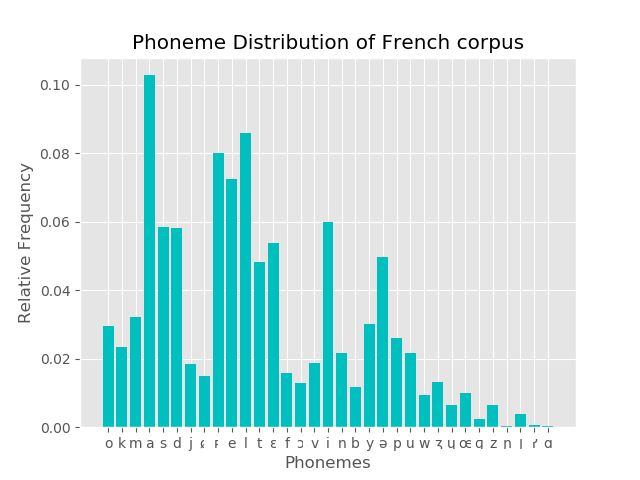
\includegraphics[keepaspectratio=true,scale=0.35]{./source/EX1.1_files/French.png} 
                    \label{fig:prob1_6_2}
                \end{minipage}%
                \begin{minipage}{.5\textwidth}
                    \centering
                    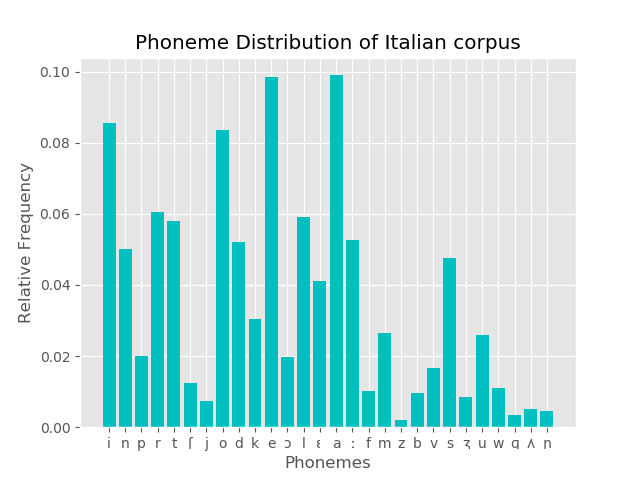
\includegraphics[keepaspectratio=true,scale=0.35]{./source/EX1.1_files/Italian.png}   
                    \label{fig:prob1_6_2}
                \end{minipage}
        \end{figure}
        
    \item[c)]
    KL Divergence is computed for each corpus using the given formula which returns value in bits 
    \\\\\\
    \item[d)]  
        From the table below we can analyze the closeness of the phonemes of different language pair from their respective probability distribution. Similarity between same corpus is $100\%$ that is why in the table for the pair X*X the dissimilarity is 0. English phonemes are more closer to French than the others, Spanish are closer to Italian whereas, French is 1.6133101058269301 bits dissimilar to the Italian which is the closest from French to Italian. Italian is the closest to Spanish. However, we can not say vice versa. For example, we already analyzed that English phonemes are more closer to French than the others, but the opposite, French phonemes are more closer to English than the others does not hold. Because we already mentioned above that French phonemes have less dissimilarity with the Italian. So the value in the table English*French = 2.8261536675741468 bits and the value French*English = 2.4309552665208773 bits do not match. Hence, the asymmetric property of the KL-divergence is justified.
        \begin{table}[ht]
            \centering
            \begin{tabular}{|c| c| c| c| c|}
                \hline 
                & English & Spanish & French & Italian \\ [0.5ex]
                \hline
                English & 0.0 & 3.4527781919333425 & 2.8261536675741468 & 3.1871598716598757\\
                \hline
                Spanish & 2.5457803433370376 & 0.0 & 1.3777115939406528 & 1.1271537967399012 \\
                \hline
                French & 2.4309552665208773 & 2.296411824471215 & 0.0 & 1.6133101058269301 \\
                \hline
                Italian & 1.8778719008184726 & 1.0740189099914261 & 1.1985568480541144 & 0.0   \\ [1ex]
                \hline
            \end{tabular}
            \caption{\hspace*{4.0cm}Table: KL Divergence for all language pair}
        \end{table}
        \end{itemize}


\section{Language Models Evaluation}
\subsection{LM Evaluation - Perplexity}
\begin{itemize}
	\item[a)]
		$$perplaxity(\mathcal{V}) = 2^{-log(\frac{1}{M})}$$
	\item[c)]
		\begin{table}
		\begin{adjustbox}{width=\columnwidth,center}
		\begin{tabular}{|c|c|c|c||c|c|c|c|}
		\hline
		\multicolumn{4}{|c||}{simplet.test}&\multicolumn{4}{c|}{wiki.test}\\\hline\hline
		\multicolumn{2}{|c|}{unigram}&\multicolumn{2}{c||}{bigram}&\multicolumn{2}{c|}{unigram}&\multicolumn{2}{c|}{bigram}\\\hline
		smoothed & unsmoothed & smoothed & unsmoothed &smoothed & unsmoothed & smoothed & unsmoothed\\\hline
		1163&no result &915&no result&1860&no result&1788&no result\\\hline 
		\end{tabular}
		\end{adjustbox}
		\end{table}
		The table shows that the peplexity of the bigrams is in both cases lower that the perplexity of the unigrams. It was not possible to calculate the perplexity for alpha = 0 because, there are several words which are not in the learned vocabulary which results in a probability of 0 or a history of 0. Both cases lead to log(0) or divsion by zero which can not be calculated. For N untrained words with a theoretical very small probability we have N times $log(1/M)$ in our sum. This explaines the high values on these unknown test corpus. 
		\item[d)]
		File simple.test has 1.96\% unseen unigrams and 18.95\% unseen bigrams.\\
		File wiki.test has 7.75\% unseen unigrams and 31.42\% unseen bigrams.\\
		The higher amount of unseen data in wiki.test explaines the higher perplexity values in the table of c), which is given by the fact that each time a new word is found the log of a realy small value gets added in the sum.
		\item[e)]
		The plots show that a bigger alpha in the smoothing changes the perplexity of the bigrams. The unigrams dont change that much in comparission with the bigram values. The important thing is that while the uniram values drop with a higher alpha, the bigram values rise with bigger alpha. The scale of this changes is bound to the amount of unseen data in the test corpus.
		\includegraphics[width=\textwidth]{source/simple_test_perplexity}
		\includegraphics[width=\textwidth]{source/wiki_test_perplexity}
		\item[f)] In the book the difinition is `a perplexity of k means that you are as surprised
on average as you would have been if you had had to guess between
k equiprobable choices at each step.'\\
The definition on this exercise sheet is the sum of the logarithms of the individual likelihood for each word and then again the log gets reversed. So the definition would be something like the normalized avarage likelihood of all the words.
\end{itemize}
\end{document}
